\documentclass[document.tex]{subfiles} 
\begin{document}

\clearpage\section{Форматы отображения схемотехнических устройств}
В разделе представлены способы использования библиотеки для формирования
синтезируемых устройств в различных видах посредством задействования механизма
адаптеров. Основные два способа отображения синтезированных устройств --
текстовый и графический.
\subsection{Отображение в формате MATLAB / Simulink}
Адаптеры, отвечающие за формирование кода модели Simulink из синтезируемых
устройств, именуются MatlabAdapter и ExtendedMatlabAdapter для генерации
отдельного блока и полноценной модели, соответственно. Описание первого
представлено в листинге~\ref{lst:matlab}.

\begin{listing}[ht]
\begin{minted}[linenos=true]{python}
class MatlabAdapter(AbstractAdapter):
    public_methods = ('matlab_code',)
    default_method = lambda self: '\n'.join(self.matlab_code())
\end{minted}
\caption{Программное описание класса адаптера MATLAB}
\label{lst:matlab}
\end{listing}

Описание расширенного адаптера для генерации моделей MATLAB / Simulink,
представленное в листинге~\ref{lst:extmatlab}, не сильно отличается от первого,
так как расширяет только функционал (здесь опущен), а не сигнатуры.
\begin{listing}[ht]
\begin{minted}[linenos=true]{python}
class ExtendedMatlabAdapter(MatlabAdapter):
    pass
\end{minted}
\caption{Программное описание класса расширенного адаптера MATLAB}
\label{lst:extmatlab}
\end{listing}

\clearpage

Пример применения расширенного адаптера к устройству (в данном случае,
мультиплексором) хорошо иллюстрируется кодом, представленным в
листинге~\ref{lst:extmatlabgen}.

\begin{listing}[ht]
\begin{minted}{pycon}
>>> from circuitry.devices.mux import DeviceMux                         
>>> from circuitry.adapters.matlab.extended import ExtendedMatlabAdapter
>>>
>>> device_mux = DeviceMux(strobe_signals='v:1', address_signals='a:2',
...                        data_signals='d:4', output_signals='o:1',
...                        strobe_signals_subs=dict(v0=1),         
...                        output_signals_subs=dict(o0=1))
>>>
>>> matlab_code = ExtendedMatlabAdapter(device_mux).default_method()
>>> 
\end{minted}
\caption{Генерация кода MATLAB}
\label{lst:extmatlabgen}
\end{listing}

По окончании выполнения кода, в переменной matlab{\_}code будет содержаться
автоматически сгенерированный код MATLAB, представленный в
листингах~\ref{lst:extmatlabgencode1},~\ref{lst:extmatlabgencode2}~и~\ref{lst:extmatlabgencode3}.

\clearpage
\begin{listing}[ht]
\begin{minted}{matlab}
sys = 'newModel1'
new_system(sys)
open_system(sys)
sys = 'newModel1/straight'
pos = [100 0 100 + 70 0 + 120]
add_block('built-in/SubSystem', sys, 'Position', pos)
pos = [400 0 400 + 30 0 + 20]
add_block('built-in/Logical Operator', [sys '/Not1'], 'Position', pos, ...
          'Operator', 'NOT', 'Number of input ports', '1') 
pos = [400 40 400 + 30 40 + 20] 
add_block('built-in/Logical Operator', [sys '/Not2'], 'Position', pos, ... 
          'Operator', 'NOT', 'Number of input ports', '1')
pos = [200 0 200 + 30 0 + 10]
add_block('built-in/Inport', [sys '/v0'], 'Position', pos)
pos = [400 80 400 + 30 80 + 20]
add_block('built-in/Logical Operator', [sys '/Not3'], 'Position', pos, ...
          'Operator', 'NOT', 'Number of input ports', '1')
pos = [400 120 400 + 30 120 + 20]
add_block('built-in/Logical Operator', [sys '/Not4'], 'Position', pos, ...
          'Operator', 'NOT', 'Number of input ports', '1')
pos = [400 160 400 + 30 160 + 20]
add_block('built-in/Logical Operator', [sys '/Not5'], 'Position', pos, ...
          'Operator', 'NOT', 'Number of input ports', '1')
pos = [400 200 400 + 30 200 + 20]
add_block('built-in/Logical Operator', [sys '/Not6'], 'Position', pos, ...
          'Operator', 'NOT', 'Number of input ports', '1')
pos = [200 30 200 + 30 30 + 10]
add_block('built-in/Inport', [sys '/a0'], 'Position', pos)
pos = [200 60 200 + 30 60 + 10]
add_block('built-in/Inport', [sys '/a1'], 'Position', pos)
pos = [200 90 200 + 30 90 + 10]
add_block('built-in/Inport', [sys '/d0'], 'Position', pos)
pos = [200 120 200 + 30 120 + 10]
add_block('built-in/Inport', [sys '/d1'], 'Position', pos)
pos = [200 150 200 + 30 150 + 10]
add_block('built-in/Inport', [sys '/d2'], 'Position', pos)
pos = [200 180 200 + 30 180 + 10]
add_block('built-in/Inport', [sys '/d3'], 'Position', pos)
pos = [600 270 600 + 30 270 + 70]
add_block('built-in/Logical Operator', [sys '/And1'], 'Position', pos, ...
          'Operator', 'AND', 'Number of input ports', '6')
pos = [600 360 600 + 30 360 + 70]
add_block('built-in/Logical Operator', [sys '/And2'], 'Position', pos, ...
          'Operator', 'AND', 'Number of input ports', '6')
pos = [600 450 600 + 30 450 + 70]
add_block('built-in/Logical Operator', [sys '/And3'], 'Position', pos, ...
          'Operator', 'AND', 'Number of input ports', '6')
pos = [800 270 800 + 30 270 + 50]
add_block('built-in/Logical Operator', [sys '/Or1'], 'Position', pos, ...
          'Operator', 'OR', 'Number of input ports', '4')
pos = [600 540 600 + 30 540 + 70]
add_block('built-in/Logical Operator', [sys '/And4'], 'Position', pos, ...
          'Operator', 'AND', 'Number of input ports', '6')
pos = [1000 660 1000 + 30 660 + 30]
add_block('built-in/Logical Operator', [sys '/And5'], 'Position', pos, ...
          'Operator', 'AND', 'Number of input ports', '2')
\end{minted}
\caption{Сгенерированный код MATLAB -- часть 1}
\label{lst:extmatlabgencode1}
\end{listing}

\clearpage

\begin{listing}[ht]
\begin{minted}{matlab}
pos = [1200 660 1200 + 30 660 + 20]
add_block('built-in/Outport', [sys '/Out1'], 'Position', pos)
add_line(sys, 'And5/1', 'Out1/1', 'autorouting','on')
add_line(sys, 'a1/1', 'Not1/1', 'autorouting','on')
add_line(sys, 'a1/1', 'And2/1', 'autorouting','on')
add_line(sys, 'a1/1', 'And1/1', 'autorouting','on')
add_line(sys, 'Not1/1', 'And4/1', 'autorouting','on')
add_line(sys, 'Not1/1', 'And3/1', 'autorouting','on')
add_line(sys, 'Not2/1', 'And4/2', 'autorouting','on')
add_line(sys, 'Not2/1', 'And2/2', 'autorouting','on')
add_line(sys, 'And1/1', 'Or1/1', 'autorouting','on')
add_line(sys, 'And2/1', 'Or1/2', 'autorouting','on')
add_line(sys, 'And3/1', 'Or1/3', 'autorouting','on')
add_line(sys, 'v0/1', 'And5/1', 'autorouting','on')
add_line(sys, 'a0/1', 'Not2/1', 'autorouting','on')
add_line(sys, 'a0/1', 'And3/2', 'autorouting','on')
add_line(sys, 'a0/1', 'And1/2', 'autorouting','on')
add_line(sys, 'Not3/1', 'And4/3', 'autorouting','on')
add_line(sys, 'Not3/1', 'And3/3', 'autorouting','on')
add_line(sys, 'Not3/1', 'And1/3', 'autorouting','on')
add_line(sys, 'Not4/1', 'And2/3', 'autorouting','on')
add_line(sys, 'Not4/1', 'And4/4', 'autorouting','on')
add_line(sys, 'Not4/1', 'And3/4', 'autorouting','on')
add_line(sys, 'Or1/1', 'And5/2', 'autorouting','on')
add_line(sys, 'Not5/1', 'And2/4', 'autorouting','on')
add_line(sys, 'Not5/1', 'And3/5', 'autorouting','on')
add_line(sys, 'Not5/1', 'And1/4', 'autorouting','on')
add_line(sys, 'Not6/1', 'And4/5', 'autorouting','on')
add_line(sys, 'Not6/1', 'And2/5', 'autorouting','on')
add_line(sys, 'Not6/1', 'And1/5', 'autorouting','on')
add_line(sys, 'And4/1', 'Or1/4', 'autorouting','on')
add_line(sys, 'd2/1', 'Not3/1', 'autorouting','on')
add_line(sys, 'd2/1', 'And2/6', 'autorouting','on')
add_line(sys, 'd3/1', 'Not4/1', 'autorouting','on')
add_line(sys, 'd3/1', 'And1/6', 'autorouting','on')
add_line(sys, 'd0/1', 'Not5/1', 'autorouting','on')
add_line(sys, 'd0/1', 'And4/6', 'autorouting','on')
add_line(sys, 'd1/1', 'Not6/1', 'autorouting','on')
add_line(sys, 'd1/1', 'And3/6', 'autorouting','on')
\end{minted}
\caption{Сгенерированный код MATLAB -- часть 2}
\label{lst:extmatlabgencode2}
\end{listing}

\clearpage

\begin{listing}[ht]
\begin{minted}{matlab}
sys = 'newModel1'
pos = [20 20 20 + 20 20 + 20]
add_block('built-in/Constant', [sys '/v0'], 'Position', pos, ...
          'Value', '1', 'OutDataTypeStr', 'boolean')
add_line(sys, 'v0/1', 'straight/1', 'autorouting','on')
pos = [20 60 20 + 20 60 + 20]
add_block('built-in/Constant', [sys '/a0'], 'Position', pos, ...
          'Value', '0', 'OutDataTypeStr', 'boolean')
add_line(sys, 'a0/1', 'straight/2', 'autorouting','on')
pos = [20 100 20 + 20 100 + 20]
add_block('built-in/Constant', [sys '/a1'], 'Position', pos, ...
          'Value', '0', 'OutDataTypeStr', 'boolean')
add_line(sys, 'a1/1', 'straight/3', 'autorouting','on')
pos = [20 140 20 + 20 140 + 20]
add_block('built-in/Constant', [sys '/d0'], 'Position', pos, ...
          'Value', '1', 'OutDataTypeStr', 'boolean')
add_line(sys, 'd0/1', 'straight/4', 'autorouting','on')
pos = [20 180 20 + 20 180 + 20]
add_block('built-in/Constant', [sys '/d1'], 'Position', pos, ...
          'Value', '0', 'OutDataTypeStr', 'boolean')
add_line(sys, 'd1/1', 'straight/5', 'autorouting','on')
pos = [20 220 20 + 20 220 + 20]
add_block('built-in/Constant', [sys '/d2'], 'Position', pos, ...
          'Value', '0', 'OutDataTypeStr', 'boolean')
add_line(sys, 'd2/1', 'straight/6', 'autorouting','on')
pos = [20 260 20 + 20 260 + 20]
add_block('built-in/Constant', [sys '/d3'], 'Position', pos, ...
          'Value', '0', 'OutDataTypeStr', 'boolean')
add_line(sys, 'd3/1', 'straight/7', 'autorouting','on')
pos = [250 20 250 + 70 20 + 30]
add_block('built-in/Display', [sys '/Display_straight_1'], 'Position', pos)
add_line(sys, 'straight/1', 'Display_straight_1/1', 'autorouting','on')
\end{minted}
\caption{Сгенерированный код MATLAB -- часть 3}
\label{lst:extmatlabgencode3}
\end{listing}

\clearpage

Модель Simulink, получаемая в результате выполнения этого кода представлена на
рисунке~\ref{fig:adapters_matlab_model}.

\begin{figure}[here]
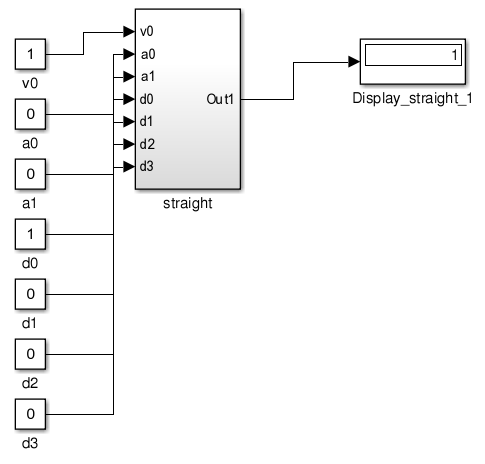
\includegraphics[width=1\linewidth]{adapters_matlab_model}
\caption{Модель мультиплексора в Simulink}
\label{fig:adapters_matlab_model}
\end{figure}

\clearpage

Блок Simulink представляет из себя схему устройства, построенную с помощью
адаптера графов (рисунок~\ref{fig:adapters_matlab_model_in}).

\begin{figure}[here]
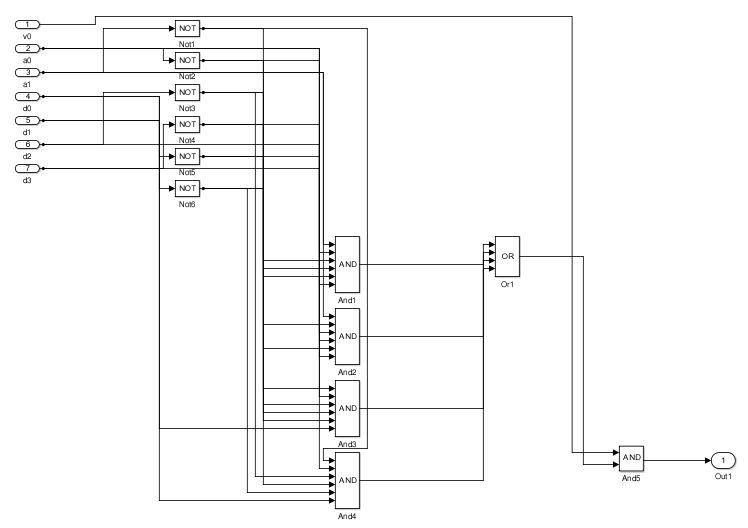
\includegraphics[width=1\linewidth]{adapters_matlab_model_in}
\caption{Модель мультиплексора в Simulink - внутреннее представление блока}
\label{fig:adapters_matlab_model_in}
\end{figure}

\end{document}